The reconstruction of ancestral languages depends on regularities that persist across phonological evolution. Sound change occurs according to consistent patterns that affect entire grammatical systems. These patterns allow historical inference to proceed by rule-governed comparison. When daughter languages show aligned differences in equivalent words, the shape of the ancestral form can often be inferred with precision.

Historical linguistics considers shared morphological and syntactic structures as indicators of genealogical descent. Correspondences in case endings, agreement systems, and word order provide signals of common ancestry. These features must appear across lexical items to count as evidence for descent. Chance resemblance or cultural borrowing cannot produce such system-wide alignment.

Proto-Indo-European (PIE) is the name assigned to the unattested language reconstructed from parallels among Indo-European languages. Its existence is inferred from regularities in grammar and phonology shared by Sanskrit, Ancient Greek, Latin, Hittite, Old Church Slavonic, and others. These languages exhibit consistent transformations that converge on reconstructed PIE forms, reflecting their shared ancestry.

The comparative method identifies sound correspondences that link descendant languages to a shared root. For example, Latin \emph{f}, Sanskrit \emph{bh}, and English \emph{b} align in inherited words, implying a common source consonant in PIE. Such correspondences must be supported by examples across word families. Once established, they allow reconstruction of ancestral forms that conform to a phonological system.

Phonological transformations affect all levels of morphology, including declensions, conjugations, and derivational patterns. These shifts are governed by well-defined constraints such as syllable structure, stress placement, and adjacent sounds. A given transformation applies across the lexicon once its domain is defined. This internal consistency permits reconstructions that are testable.

Kinship terms, natural elements, and tools form high-retention vocabulary with cross-linguistic stability. These words resist borrowing, undergo regular phonological change, and remain semantically intact across time scales. They serve as indicators of shared ancestry in historical reconstruction.

The PIE root \piefont{*dʰugh₂tḗr}, meaning "daughter," provides one of the clearest examples of stability across Indo-European languages. Despite phonological divergence, the kinship meaning is retained with consistency from Vedic Sanskrit to modern English.

In Sanskrit, the form is \textsanskrit{दुहितृ} (\emph{duhitṛ}), preserving both the root and the feminine suffix. Ancient Greek gives \textgreek{θυγάτηρ} (\emph{thygatēr}) — where the initial aspirated dental is retained. Latin replaced the expected cognate of PIE \piefont{*dʰugh₂tḗr} with \emph{filia}, from an entirely different root meaning "suckling" (related to \emph{filius} for "son"). In Gothic, the reflex is \emph{dauhtar}, leading to Old English \emph{dohtor} and eventually modern English "daughter."

These forms are an example of predictable sound changes. The PIE voiced aspirated dental \piefont{*dʰ} becomes \emph{th} in Greek and \emph{d} in Germanic. The laryngeal \piefont{*h₂} affects surrounding vowels and often disappears. Preservation of suffixes and semantic continuity reinforce the reconstruction's accuracy.

A second example, drawn from material instead of kinship vocabulary, illustrates the principles of retention and transformation. The PIE root \piefont{*kʷékʷlos}, meaning "wheel" or "circle," illustrates how this root produced enduring derivatives across Indo-European languages. Across language families, this root led to distinct yet semantically linked terms for circularity and motion.

In Greek, \textgreek{κύκλος} (\emph{kyklos}) retained the meanings of "circle" and "wheel," later influencing Latin \emph{cyclus} and English "cycle." Sanskrit preserved the root as \textsanskrit{चक्र} (\emph{chakra}), initially referring to a physical wheel, and later extended to cycles in philosophical and spiritual contexts. In Proto-Germanic, the root evolved into \piefont{*hweulą}, producing Old English \emph{hweol}, Middle English \emph{whele}, and modern English "wheel."

Phonological shifts altered the surface form, but the meaning remained around rotation and recurrence. Latin \emph{colere}, meaning "to cultivate" or "to tend," may derive from \piefont{*kʷel-} ("to turn") — though this etymology remains speculative — generating \emph{cultus} ("ritual care") and eventually "cult." A related case is Latin \emph{circulus}, a diminutive of \emph{circus} ("ring"), which became English "circle" via Old French \emph{cercle}. Although derived from a separate PIE root (\piefont{*sker-}, "to bend, turn"), its semantic parallel to \textgreek{κύκλος} reflects linguistic convergence.

In Semitic languages, comparable formations are found. Hebrew \texthebrew{גלגל} (\emph{galgal}), meaning "wheel" or "rolling object," derives from the root \emph{g-l-l}, which denotes circular motion. Related terms include \texthebrew{גל} (\emph{gal}, "wave"), \texthebrew{גללים} (\emph{galalim}, "dung pellets"), and \texthebrew{גולגולת} (\emph{gulgoleth}, "skull"). The reduplication in \emph{galgal} superficially resembles the PIE form \piefont{*kʷékʷlos} (\piefont{kʷe-kʷl-os}), but the similarity is incidental, as these forms derive from distinct morphological systems.

Reduplication as a strategy for emphasizing repetition or motion appears independently across language families. Its presence in both Indo-European and Semitic systems points to a broader cross-linguistic pattern. The recurrence of phonemes, as in \texthebrew{גלגל} and \piefont{*kʷékʷlos}, reinforces the idea of circularity through sound. Just as the wheel itself arose independently in different cultures, linguistic forms encoding rotation also emerged separately.

The comparative method excludes false cognates. Consider English "day" and Latin \emph{dies} — both refer to a 24-hour period and share similar sounds, yet they derive from entirely unrelated PIE roots.

English "day" traces back through Old English \emph{dæg} to PIE \piefont{*dʰegʷʰ-}, meaning "to burn" or "to be hot." The semantic connection runs from the heat of daylight to the daylight period itself. In contrast, Latin \emph{dies} descends from PIE \piefont{*dyéws}, meaning "sky" or "to shine," related to \emph{deus} ("god") and Sanskrit \emph{dyáus} ("sky, heaven"). Both roots metaphorically extended to "day," but through independent pathways.

The comparative method distinguishes such cases by requiring regular sound correspondences across word families. English "day" follows Germanic sound laws: PIE \piefont{*dʰ} regularly becomes \emph{d} in English, and \piefont{*gʷʰ} becomes \emph{g} (later weakened to zero). Latin \emph{dies}, however, shows the expected Latin treatment of PIE \piefont{*dy}: the sequence becomes \emph{di-} in Latin, as seen in \emph{Iovis} (Jupiter) from \piefont{*dyēws}.

Had these words been genuine cognates, we would expect to find the same root appearing across Romance and Germanic languages with parallel semantic development. Instead, we find that other Germanic languages show the \piefont{*dʰegʷʰ-} root (German \emph{Tag}, Dutch \emph{dag}), while Romance languages consistently reflect \piefont{*dyéws} (French \emph{jour} from Latin \emph{diurnus}, Spanish \emph{día}). The pattern confirms separate origins despite surface similarity.

Another case involves English "much" and Spanish "mucho" — words that are nearly identical in sound and meaning yet stem from unrelated PIE roots. English "much" derives from Old English \emph{micel} and ultimately PIE \piefont{*méǵh₂s} ("great"), whose Latin cognate is \emph{magnus}. Spanish "mucho," however, comes from Latin \emph{multus} ("many"), which traces to PIE \piefont{*mel-} ("strong"). The superficial resemblance results from convergent phonological development: Germanic \piefont{*k} > English \emph{ch}, and Latin consonant clusters \emph{-lt-} > Spanish \emph{ch}. The true English cognate of "mucho" would be a derivative of \emph{magnus}, while the Spanish cognate of "much" appears in \emph{más} (from Latin \emph{magis}).

This systematic approach prevents the method from accepting coincidental resemblances, borrowings, or parallel semantic developments. True cognates must satisfy constraints simultaneously: sound correspondences, morphological patterns, and semantic plausibility across the language family. 

\begin{commentary}[Commentary: A Personal Encounter]
At thirteen, I spent lunch breaks calling the Academy of the Hebrew Language from a pay phone, taking advantage of their public consultation hours. One question preoccupied me: the meaning of the Hebrew phrase \texthebrew{וחוזר חלילה} (\emph{vechozer chalilah}). The expression denotes endless repetition, "again and again" or "in a cycle," yet the word \texthebrew{חלילה} (\emph{chalilah}) also means "God forbid." Why would a phrase about recurrence contain a word implying prohibition?

The Academy asked for two weeks to investigate. When I called again, they proposed three hypotheses. One traced it to \texthebrew{חלל} (\emph{chalal}, "void"), implying unboundedness. Another derived it from \texthebrew{חול} (\emph{chol}, "sand"), whose accumulation metaphorically signals continuity. A final suggestion pointed to \texthebrew{חליל} (\emph{chalil}, "flute"), possibly named for its cylindrical form.

None of these answers resolved my curiosity. Years later, I encountered \piefont{*kʷékʷlos} and its descendants: \textgreek{κύκλος} (\emph{kyklos}), \textsanskrit{चक्र} (\emph{chakra}), "cycle," and "wheel." I remembered that call. Across language families, words for turning often imply repetition.

Sound plays a role. Words like \texthebrew{חלילה} (\emph{chalilah}) and \texthebrew{גלגל} (\emph{galgal}) echo themselves, as do Greek \textgreek{ροίζος} (\emph{rhoizos}, "whirring noise") and other motion-related terms. Reduplication strengthens the perception of rotation. Whether \texthebrew{וחוזר חלילה} originated independently or reflects a linguistic universal, it illustrates a principle: what turns, returns.

Years later, at the Technion, I worked in an EEG lab run by Professor Hillel Pratt, a scientist of towering breadth and compassion. Our conversations drifted across neuroscience, etymology, and Aramaic grammar. For over a couple of years, we debated word origins.

Then one day I learned he was a sitting member of the Academy of the Hebrew Language. He had never mentioned it. He let the ideas speak for themselves. Technically, he was \textit{always} right.
\end{commentary}

\begin{figure}[htbp]
\centering
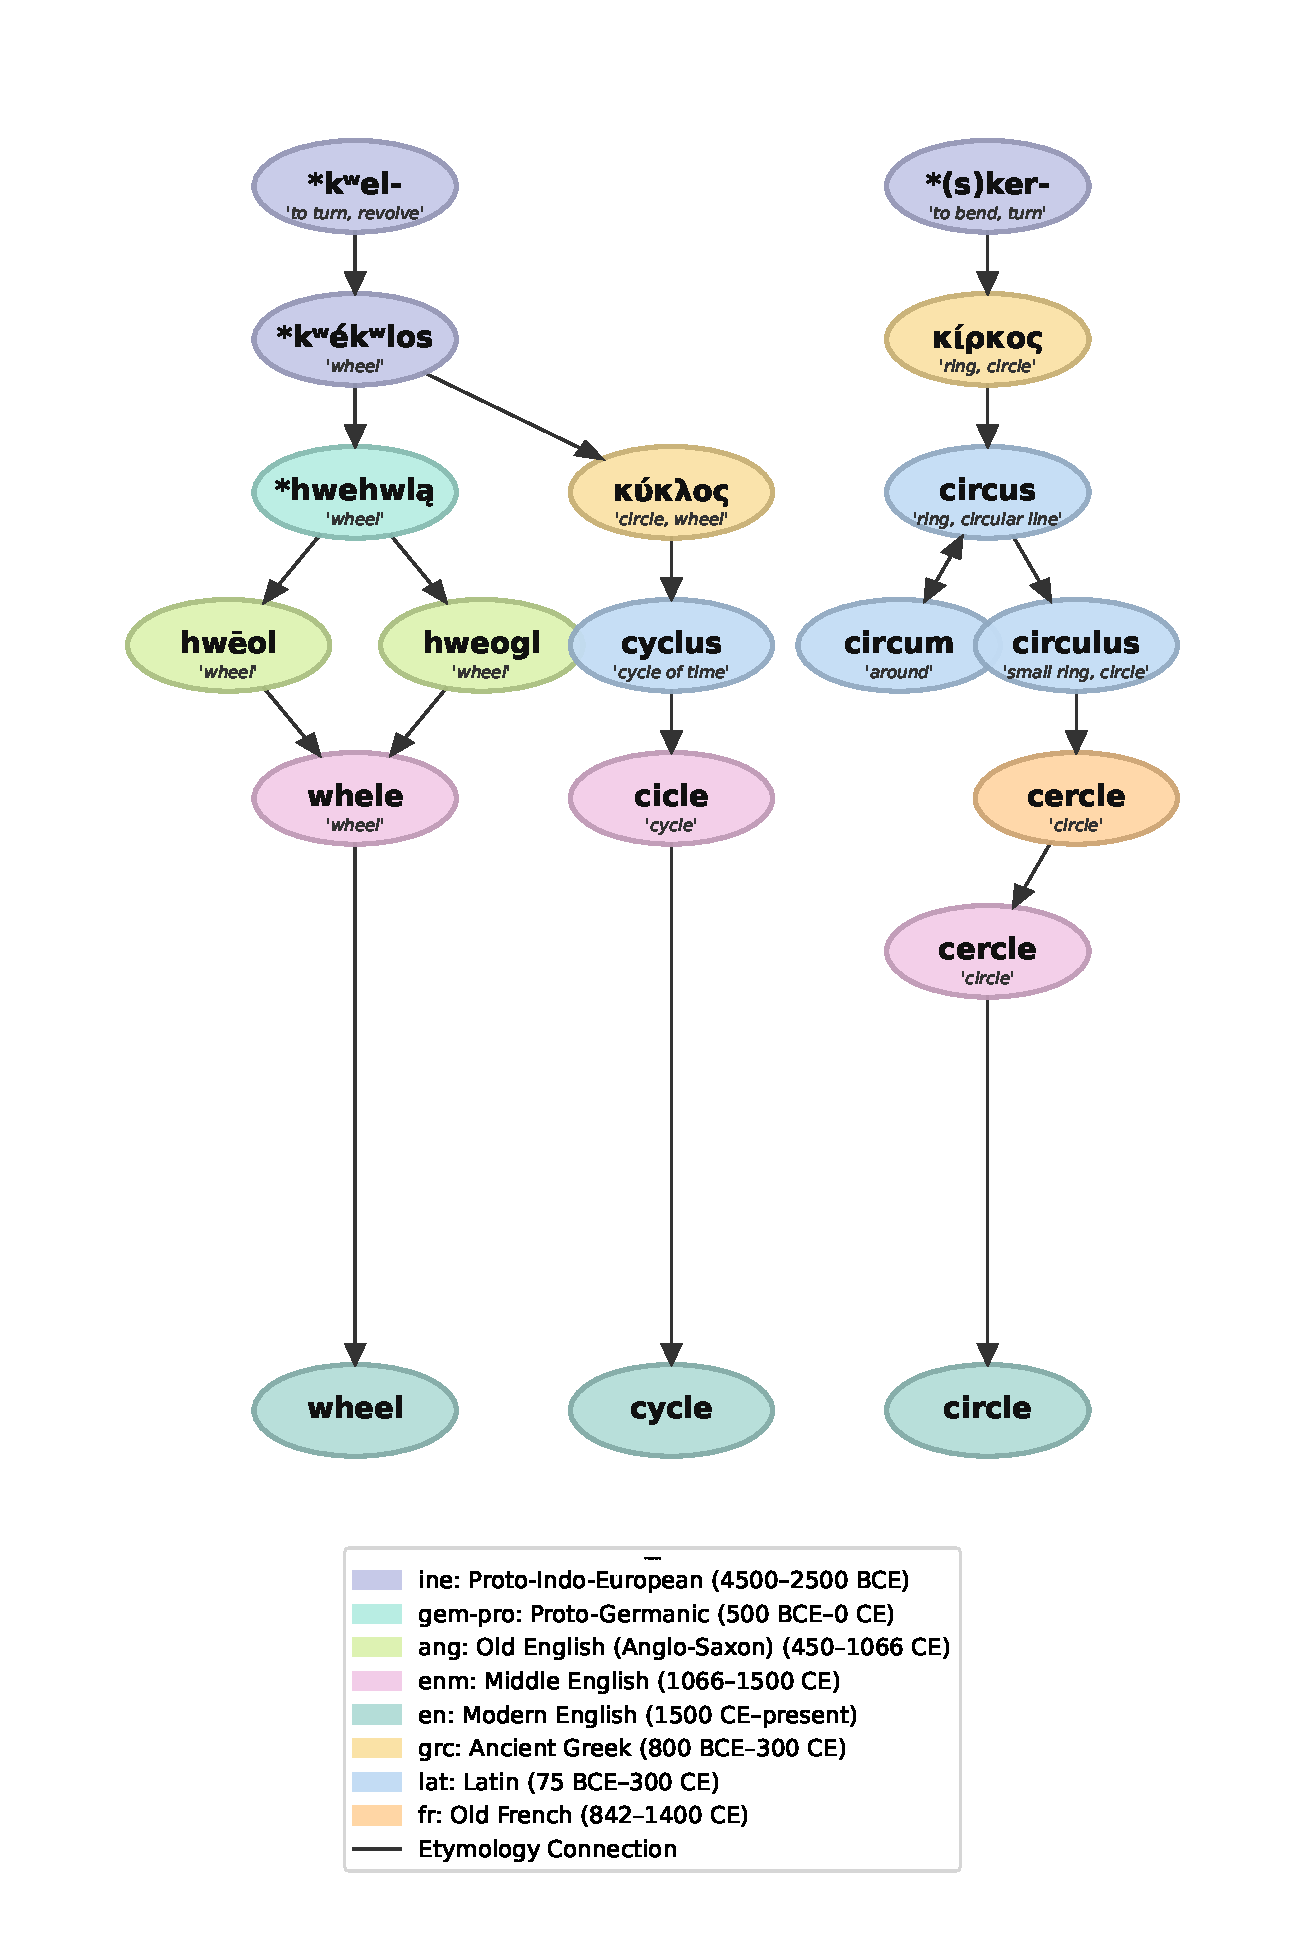
\includegraphics[width=0.85\textwidth,height=0.75\textheight,keepaspectratio]{05_CircleWheel/etymology_graph_portrait_v105.pdf}
\caption*{Etymological relationships in the Indo-European family showing the evolution of the PIE root \piefont{*kʷékʷlos} ("wheel, circle") across major language branches. The diagram illustrates systematic phonological transformations: de-labialization in Latin (\emph{colere}) versus preservation as \emph{qu} (e.g., \emph{equus}, \emph{quattuor}), palatalization in Sanskrit (\emph{chakra}), contextual neutralization in Greek (\emph{kyklos}), and fricativization through Grimm's Law in Germanic (\emph{wheel}). Color coding distinguishes language families while maintaining visual clarity of the genealogical relationships that underlie comparative reconstruction.}
\end{figure}
